\documentclass[wide,a4paper,titlepage,12pt] {article}
\usepackage{polski}
\usepackage[utf8]{inputenc}
\usepackage{listings}
\usepackage{slashbox}
\usepackage[table]{xcolor}
\usepackage{graphicx,pdflscape}
\usepackage{placeins}

\title{Układy cyfrowe i systemy wbudowane}
\author{Tymon Tobolski (181037)\\ Jacek Wieczorek (181043)}

% Title page layout (fold)
\makeatletter
\renewcommand{\maketitle}{
\begin{titlepage}
  \begin{center}
    \vspace*{3cm}
    \LARGE \@title \par
    \vspace{2cm}
    \textit{\small Autor:}\par
    \normalsize \@author\par \normalsize
    \vspace{3cm}
    \textit{\small Prowadzący:}\par
    Dr inż. Jarosław Sugier \par
    \vspace{2cm}
    Wydział Elektroniki\\ III rok\\ Pn 14.15 - 16.00\par
    \vspace{4cm}
    \small \@date
  \end{center}
\end{titlepage}
}
\makeatother

\begin{document}
\maketitle
  \section{Cel ćwiczenia}
  Celem ćwiczenia było stworzenie układu generującego sygnał prostokątny o zadanym przebiegu.
  Układ składał się z dwóch podukładów: licznika "0-7" oraz dekodera "1 z 8".
  Oba podukłady zostały zaimplementowane jako osobne urządzenia, a następnie użyte w głównym układzie.

  \begin{figure}[htbp]
    \begin{center}
      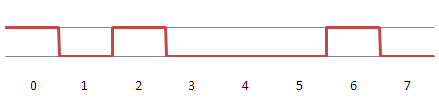
\includegraphics[scale=0.5]{syg.png}
      \caption{Przebieg sygnału}
    \end{center}
  \end{figure}

 

  \section{Licznik}

  \subsection{Licznik asynchroniczny}
  Licznik działający asynchronicznie został stworzony za pomocą trzech przerzutników typu T połączonych kaskadowo. Pierwszy przerzutnik był sterowany zegarem, pozostałe były aktywowane opadającym zboczem swojego poprzednika.

  \begin{figure}[htbp]
    \begin{center}
      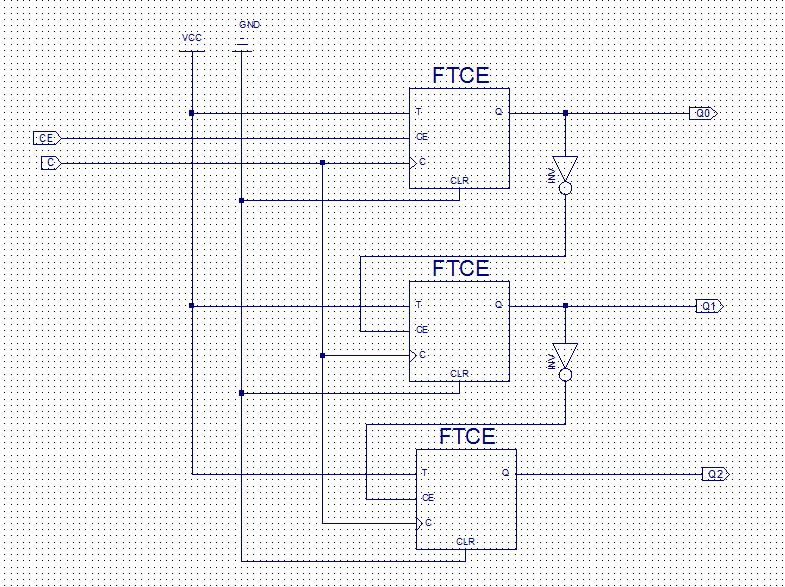
\includegraphics[scale=0.4]{licznik_asynch.png}
      \caption{Schemat licznika asynchronicznego}
    \end{center}
  \end{figure}

  \begin{figure}[htbp]
    \begin{center}
      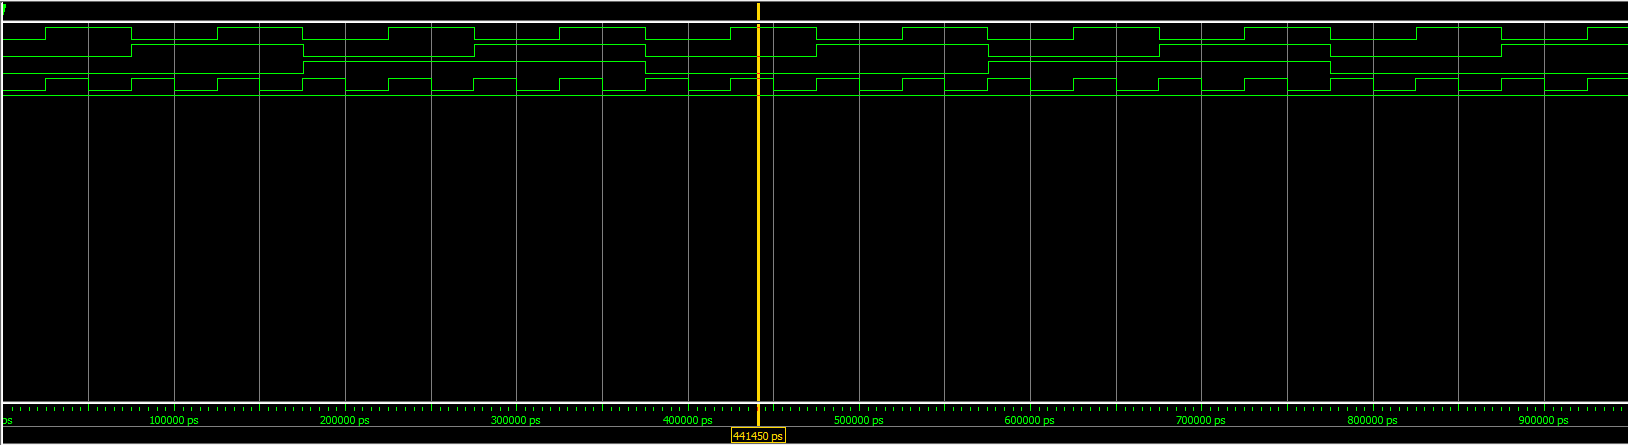
\includegraphics[scale=0.2]{licznik_beh.png}
      \caption{Symulacja behawioralna działania licznika asynchronicznego}
    \end{center}
  \end{figure}

  \newpage

  \subsection{Licznik synchroniczny}

  \begin{center}
    \begin{tabular}{|c|c|c|c|c|}
    \hline
    \backslashbox{$Q_{0}$}{$Q_{2}$$Q_{1}$} & 00 & 01 & 11 & 10 \\ \hline
    0 & 0 & 0 & \cellcolor[gray]{0.8}1 & \cellcolor[gray]{0.8}1 \\ \hline
    1 & 0 & \cellcolor[gray]{0.8}1 & 0 & \cellcolor[gray]{0.8}1 \\ \hline
    \end{tabular}
    \\ $Q_{2}'$ = $Q_{2} \bar{Q_{0}}$ + $Q_{2} \bar{Q_{1}}$ + $\bar{Q_{2}} Q_{1} Q_{0}$
  \end{center}

  \begin{center}
    \begin{tabular}{|c|c|c|c|c|}
    \hline
    \backslashbox{$Q_{0}$}{$Q_{2}$$Q_{1}$} & 00 & 01 & 11 & 10 \\ \hline
    0 & 0 & \cellcolor[gray]{0.8}1 & \cellcolor[gray]{0.8}1 & 0 \\ \hline
    1 & \cellcolor[gray]{0.8}1 & 0 & 0 & \cellcolor[gray]{0.8}1 \\ \hline
    \end{tabular}
    \\ $Q_{1}'$ = $Q_{1} \oplus Q_{0} $
  \end{center}

  \begin{center}
    $Q_{0}'$ = $\bar{Q_{0}}$
  \end{center}


  \begin{figure}[htbp]
    \begin{center}
      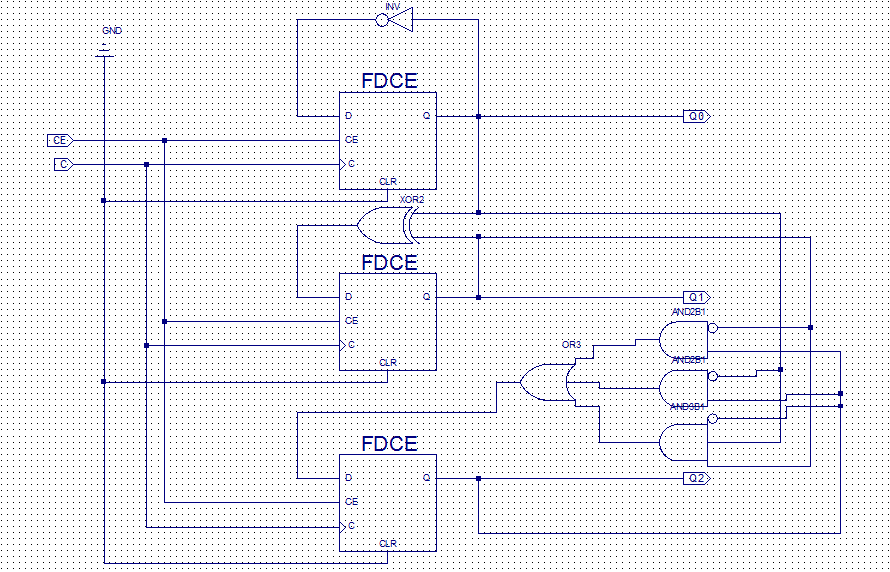
\includegraphics[scale=0.6]{licznik.png}
      \caption{Schemat licznika synchronicznego}
    \end{center}
  \end{figure}

  \newpage

  \section{Dekoder}
  Dekoder sygnału 3-bitowego na sygnał 8-bitowy został utworzony z 8 po trójnych brame AND z zanegowanymi odpowiednimi wejściami.

  \begin{figure}[htbp]
    \begin{center}
      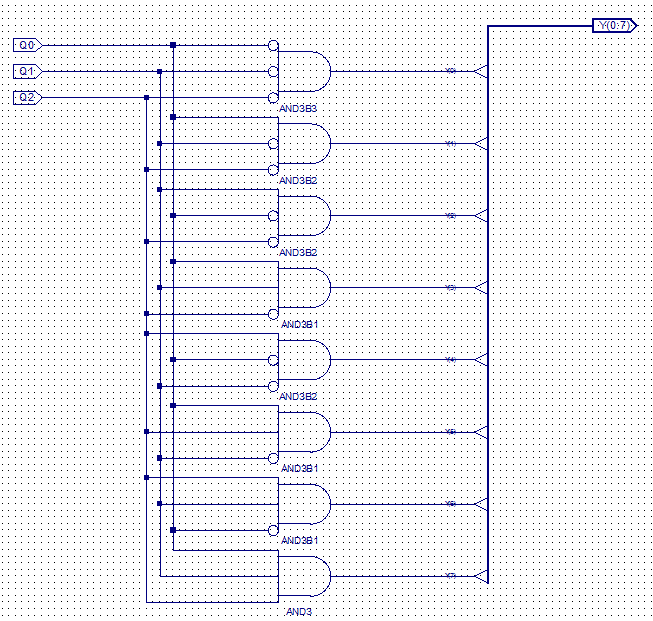
\includegraphics[scale=0.6]{dekoder.png}
      \caption{Schemat dekodera}
    \end{center}
  \end{figure}

  \begin{figure}[htbp]
    \begin{center}
      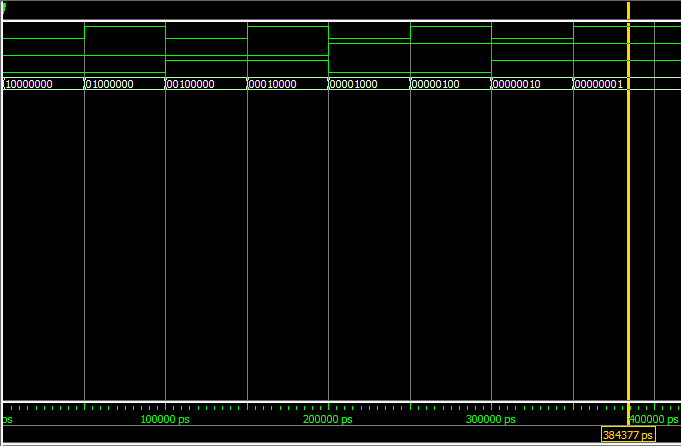
\includegraphics[scale=0.4]{dekoder_beh.png}
      \caption{Symulacja behawioralna działania dekodera}
    \end{center}
  \end{figure}

  \newpage

  \section{Generator sygnału}
  Generator został zbudowany z połączenia licznika, dekodera, a następnie potrójnej bramki OR podłączonej do 0, 2 i 6 bitu magistrali wyjścia dekodera.

  \begin{figure}[htbp]
    \begin{center}
      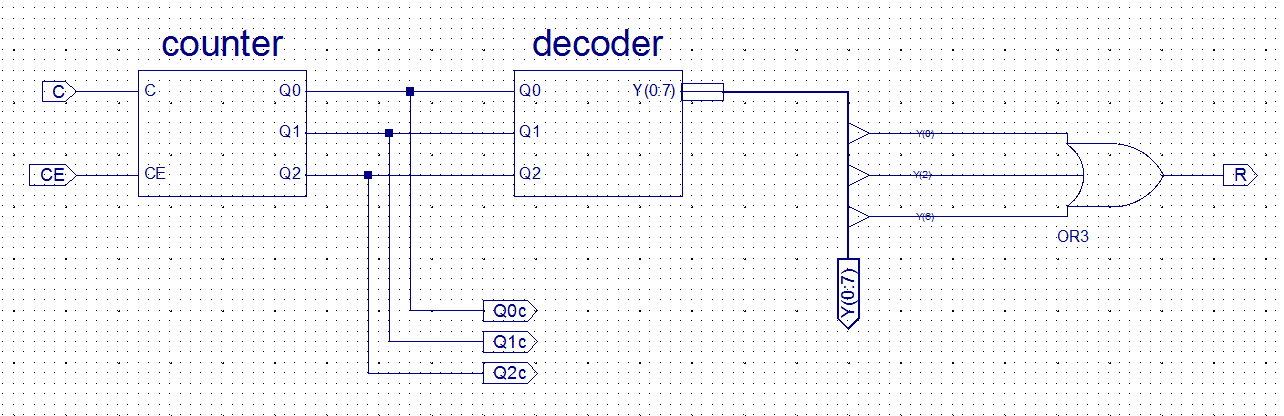
\includegraphics[scale=0.4]{uklad.png}
      \caption{Schemat gotowego układu}
    \end{center}
  \end{figure}

\newpage
\begin{landscape}

  \begin{figure}[htbp]
    \begin{center}
      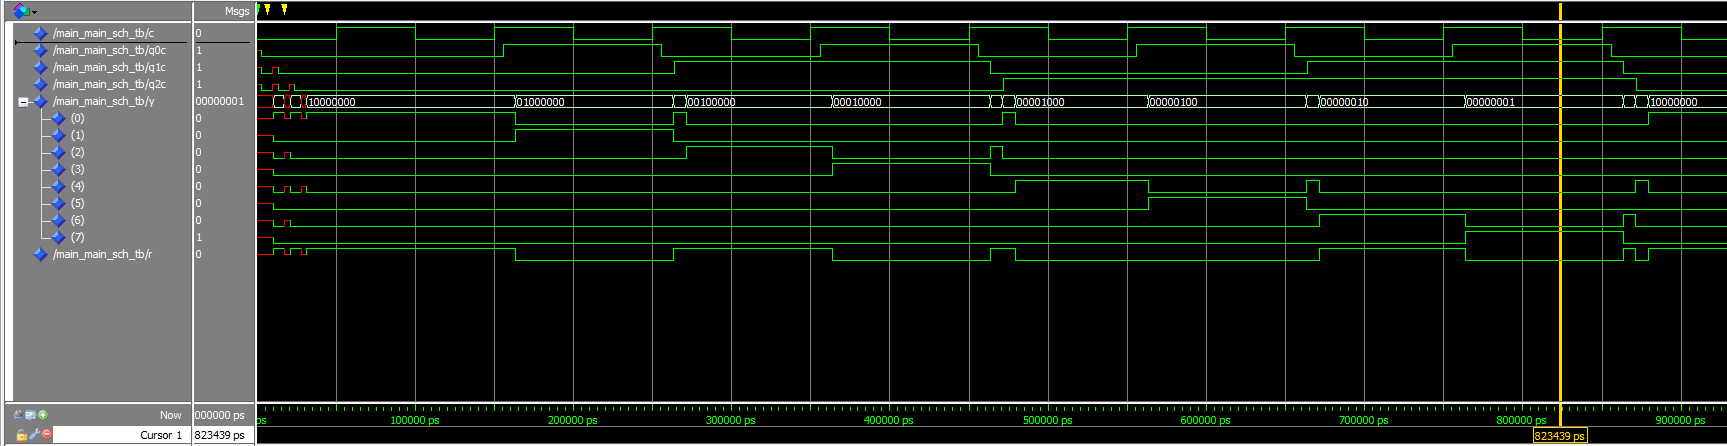
\includegraphics[scale=0.3]{ukl_asynch.png}
      \caption{Działanie układu z licznikiem asynchronicznym}
    \end{center}
  \end{figure}


  \begin{figure}[htbp]
    \begin{center}
      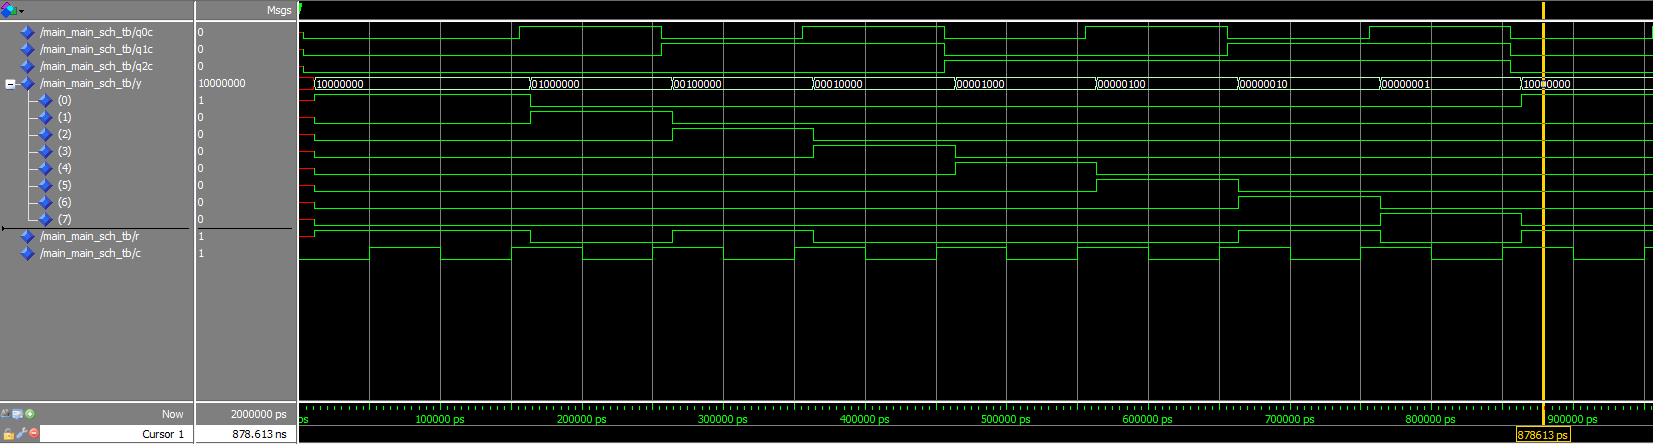
\includegraphics[scale=0.3]{ukl_synch.png}
      \caption{Działanie układu z licznikiem synchronicznym}
    \end{center}
  \end{figure}
\end{landscape}
\newpage

  \section{Wnioski}
Analiza czasowa działania układu przy zastosowaniu licznika asynchronicznego ukazuje niedokładności wynikające z opoźnien przerzutnikow. Przerzutnikii są uruchamiane kaskadowo co powoduje przekłamanie stanu układu przez krótki okres czasu. Widać to np. przy przejściu ze stanu kodującego liczbę 3 do 4. Układ na chwilę znajduje się w stanie 2, a potem 0 (dającymi wynik 1), więc dlatego pojawia się chwilowe przekłamanie. Podobna sytuacja pojawia sie przy przejściu ze stanu 7 na stan 0. Następuje to poprzez stan 6 dający wynik 1 i stan 4, dający 0. Wynikiem tego jest krótkotrwała fala wyników. Jednym ze sposobów eliminacji tego problemu jest zastosowanie licznika synchronicznego, w którym zmiana stanów następuje w tym samym momencie, nie powodując tym samym występowania "fałszywych" sekwencji przekłąmujących układ.

\end{document}



